\clearpage
\begin{summarybox}
\textbf{\textcolor{CSummary}{一句话快记}}\par
\textbf{两根看三处：判别式、对称轴、两端位置。}先确定有两个交点，再确认交点没有跑出区间。
\[\boxed{\Delta>0,\quad m<x_0<n,\quad af(m)>0,\quad af(n)>0.}\]
\begin{center}
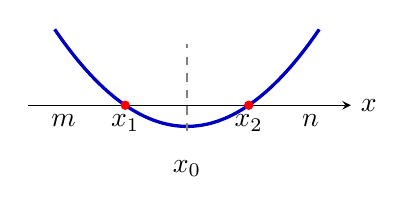
\begin{tikzpicture}[x=1.12cm,y=.83cm,>=stealth]
 \draw[->] (-1.8,0)--(1.86,0) node[right]{$x$};
 \draw[very thick,blue!75!black,domain=-1.5:1.5,samples=60] plot (\x,{.66*(\x*\x-.49)});
 \draw[dashed,gray] (0,-.4)--(0,.93);
 \node[below] at (-1.4,0) {$m$};\node[below] at (-.7,0) {$x_1$};\node[below] at (0,-.7) {$x_0$};\node[below] at (.7,0) {$x_2$};\node[below] at (1.4,0) {$n$};
 \fill[red] (-.7,0) circle(1.7pt) (.7,0) circle(1.7pt);
\end{tikzpicture}

\end{center}
\textbf{\textcolor{CSummary}{一个根要多看一眼}}\par
\begin{itemize}[leftmargin=*,itemsep=.3em]
 \item $f(m)f(n)<0$：\textbf{一定}恰有一个零点（最快用法）。
 \item 两端不异号：\textbf{不能直接断言没有一个零点}；要查$\Delta=0$且顶点在区间内，或端点是否为根且另一个根在区间内。
 \item 端点不算！两端都不是根时，恰一个零点当且仅当\textbf{两端异号或区间内有重根}。
\end{itemize}
\textbf{\textcolor{CSummary}{考试速查}}\par
求“\textbf{两不同根}”先列四个不等式，求“\textbf{恰一零点}”先异号、再重根、最后查端点。\textbf{把草图画出来，比硬背一串条件更不容易错。}
\end{summarybox}
